\section{Key techniques of \name}
\label{sec:algorithm}
We now present \name's key techniques to realize online 
adaptation of \nn configurations by harnessing the temporal
and spatial correlations of \nn performance (\S\ref{sec:insights}).

\subsection{Temporal incremental update}
\name splits the video feeds into {\em segments}, each 
of which is a set of frames of a video feed in a fine-grained 
$T$-second (by default, $T=4$) interval. 
We use $S_{i,j}$ to denote the $j^\textrm{th}$ segment of the
$i^\textrm{th}$ video.
Algorithm~\ref{alg:temporal} shows the pseudocode of \name's
temporal incremental update. 
Because of the temporal correlations of \nn performance 
(\S\ref{sec:insights}), the \nn configurations do 
not have to be re-profiled and updated for each segment.
Instead, \name first profiles a large configuration space 
every $k$ segments using the first $t$ seconds of video, and 
gets a small subset of most promising configurations (line~2).
Then, \name only profiles this subset for the rest of segments
until the next reprofiling (line~4-6).
We call the sequence of segments 
$W_{i,l}=(S_{i,kl},\dots,S_{i,k(l+1)-1})$
the $l^\textrm{th}$ {\em profile window} of 
video $i^\textrm{th}$.

\begin{algorithm}[t!]
    \small
	\DontPrintSemicolon
    \SetKwFunction{ProcessWindow}{UpdateProfileWindow}
    \SetKwFunction{Profile}{Profile}
    \SetKwProg{Fn}{Function}{:}{}
	\KwIn{$W_{i,l}$: the $l^\textrm{th}$ profile window of the
	$i^\textrm{th}$ video; $C$: all configurations under consideration}
	\KwOut{Configuration $\hat{c}_{i,j}$ for each segment $S_{i,j}$.}
    \Fn{\ProcessWindow{$W_{i,l},C$}}{
        $C_l^{promising}\leftarrow$ \Profile{$T_{i,j},C,n$}\\
        $\hat{c}_{i,j}\leftarrow C_l^{promising}[0]$\\
        \ForEach{$j=kl,\dots,k(l+1)-1$}{
            $C\leftarrow$\Profile{$T_{i,kl},C_l^{promising},1$}\\
            $\hat{c}_{i,j}\leftarrow C[0]$\\
        }
        \Return{$\hat{c}_{i,kl},\dots,\hat{c}_{i,k(l+1)-1}$}
    }
	\caption{Temporal incremental updates.}
	\label{alg:temporal}
\end{algorithm}


While profiling configuration spaces happens every $T$ segments, 
its cost may still induce a significant overhead to resource
consumption,
especially if the amount of all possible configurations grows
exponentially with more knobs.
Instead of profiling the performance of a high 
dimensional configuration space of multiple knobs, \name
updates one knob at a time while fixing the values on other
knobs.
By treating the knobs separately, we can reduce the 
re-profiling cost from $O(n^k)$ (an exhaustive search in $k$
knobs each having $n$ values) to $O(n\cdot k)$.
The insight is that 
for each knob, the relationship between its value and inference 
accuracy is independent to the setting on other knobs. 
That is, for instance, if 5fps is the least frame rate to get an F1 
score of 0.8 when the frame size is 960p, then 5fps will be the
least frame rate to attain an F1 score of 0.8 when the frame size 
is 480p.
The intuition behind the independence between knobs is that the 
impact of these knobs on accuracy is determined by {\em orthogonal} 
factors. 
For instance, in pipeline $A$, the frame rate concerns the object
moving speed, image sizes concerns the number of pixels to cover 
each object of interest, and the object detection model depends on 
whether the shape of an object can be expressed by the extracted 
features.
This allows us to profile knobs separately, and safely ignore the 
combinational effects between knobs.

\begin{algorithm}[t!]
\small
	\DontPrintSemicolon
    \SetKwFunction{Overall}{ConfigAdaptation}
    \SetKwFunction{ProfilingUnit}{Profile}
    \SetKwProg{Fn}{Function}{:}{}
	\KwIn{$n$ video feed $M_1,\dots,M_n$, and all possible configurations $C$, each being a combination of values on $k$ knobs, where $V_k$ and $v_k^*$ are the values of knob $k$ and its most expensive value.}
	\KwOut{Configuration $\hat{c}_{M_i,T_j}$ for video $M_i$ in time window $T_j$.}
% 	\Fn{\Overall{$\{M_1,\dots,M_n\}, C, \alpha$}}{
%         \ForEach{$j$-th $T$-second time window $T_j$}{
%     	    \ForEach{$M_i$}{
%         	    $X_{i,j}\leftarrow I(M_i,t_j)$\\
%         	    $\hat{c_{M_i,T_j}}\leftarrow \ProfilingUnit(X_{i,j},C,\alpha)$\\
%         	}
%     	}
%     	\Return{$\hat{c}_{M_i,T_j}$ for all $M_i$ and $T_j$}
% 	}
    \Fn{\ProfilingUnit{$X, C$}}{
        $c^{default}=(v_1^{default},\dots,v_m^{default})$\\
        \tcc{\small{Optimize one knob at a time}}
        \ForEach{Knob $k$}{
            $R_{min}\leftarrow\infty$; $A_{best}\leftarrow 1$\\
            \ForEach{$v_k\in V_k$}{
                \tcc{\small{Change only knob $k$ to $v_k$}}
                $c(v_k)\leftarrow Replace(c^{default},k,v_k)$\\
                $c(v_k^*)\leftarrow Replace(c^{default},k,v_k^*)$\\
                $A\leftarrow F(X,c(v_k),c(v_k^*))$\\
                \tcc{\small{Set knob $k$ to $v$, if $v$ is cheaper and is accurate enough}}
                \If{$R(c(v_k)) < R_{min}$ \textrm{\bf and} $A \geq \alpha$}{
                    $\hat{v_k}\leftarrow v$; $R_{min}\leftarrow R(c(v_k))$; $A_{best}\leftarrow A$\\
                }
            }
            \tcc{\small{Update the accuracy threshold}}
            $\alpha=\frac{\alpha}{A_{best}}$
        }
        \Return{$\hat{c}\leftarrow(\hat{v_1},\dots,\hat{v_n})$}
    }
	\caption{Profiling configuration knobs separately.}
	\label{alg:policy3}
\end{algorithm}

Algorithm~\ref{alg:policy3} describes how \name profiles the knobs
separately. 
Let $Replace(C,k,v)$ denote the result of setting knob $k$ of $C$ 
with $v$, and $F(X,c,c^*)=\frac{1}{|X|}\sum_{x\in X}f(x,c,c^*)$ 
denote the average F1 score of $c$ with respect to $c^*$ over a 
set of frames $X$.
For every $T$ seconds, it re-profiles and updates the 
configurations on the frames in the first $t$ seconds.
For each knob $k$, it tries all of its possible values while 
fixing other knobs to their default values $C(v_k)$, and calculate
the accuracy with respect to setting knob $k$ to its most 
expensive values as the golden
configuration $C(v_k^*)$ (line~5-7). 
This allow us to identify the ``sweet spot'' value of knob $k$ 
that has least resource consumption while achieving enough 
accuracy (line~8-9).
Finally, since the accuracy degradation of individual knobs will 
be accrued when combining them together, we increase the accuracy 
threshold after each knob is updated (line~10).
% Given a configuration $C$, configuration 
% $C'=C\setminus\{v_k\}\cup \{v_k^*\}$ has the same values to $C$ except for the $k$-th knob, on which $C$ has $v_k$ and $C^*$ has $v_k^*$.
There are two more details in online profiling.
First, for some knobs (e.g., frame rate, minimal area size), a
lower value has no profiling cost, if a higher value has been
profiled, because the output of the lower value can be extrapolated
from the output of a higher values (e.g., for frame rate, it means
simply ignoring frames in the higher frame rate output).
Second, Policy~3 depends on the default values, though different
settings of default values only yield marginal performance 
difference.~\footnote{We notice that such independence would be 
weakened in extreme cases; e.g., it is hard to profile the accuracy
of different frame rates, under too small an image size, as no \nn
would detect any objects. So when profiling a certain knob, other
knobs are not set to such extreme values.}


\subsection{Spatial cross-video inference}








\subsection{Overview}

We begin with the workflow of \name.
\name splits the video feeds into {\em segments}, each 
of which is a set of frames of a video feed in a fine-grained 
$T$-second (by default, $T=4$) interval. 
We use $S_{i,j}$ to denote the $j^\textrm{th}$ segment of the
$i^\textrm{th}$ video.
As implied by the temporal and spatial correlations of \nn 
performance (\S\ref{sec:insights}), the \nn configurations do 
not have to be re-profiled and updated for each segment.
At a high level, \name should instead use the best 
configuration(s) of one segment to ``guide'' the selection of 
the best configuration of the future segments of the same 
video and the segments of similar videos. 
To do this, \name runs a process every $k$ 
segments worth of time, called a {\em profile window}. 
We denote the $l^\textrm{th}$ profile window of video 
$i^\textrm{th}$ by $W_{i,l}=(S_{i,kl},\dots,S_{i,k(l+1)-1})$.


Figure~\ref{fig:workflow} shows an example of \name in action.
Suppose we have two similar video feeds; i.e., they share 
similar distributions of the best \nn configurations.
Say we are in the $i^\textrm{th}$ profile time window.
\begin{packeditemize}
\item {\bf Periodic re-profiling:}
\name begin by profiling the performance of many configurations 
on the first $t$ seconds of $W_{i,1}$ to identify
a small set of ``most promising''configurations (the set only has
one element in the example).
\item {\bf  Temporal incremental update:} 
For each Video~\#1 segment between two re-profiling events, 
\name will first apply a {\em light-weight check} on the first 
$t$ seconds to decide which of the configurations in the set is 
the cheapest and accurate (with respect to the accuracy 
threshold $\alpha$), and use that configuration for the rest of 
the segment.
\item {\bf Spatial cross-video inference:}
Since we already know the most promising configurations of a 
similar video feed (Video~\#1), we can simply choose the best 
configuration of Video~\#2 from this set;
operationally, in each segment of Video~\#2, we will apply the
light-weight check to identify which of the most promising 
configurations of Video~\#1 is the cheapest yet  accurate 
configuration of Video~\#2.
\end{packeditemize}

\begin{figure}[t!]
\centering
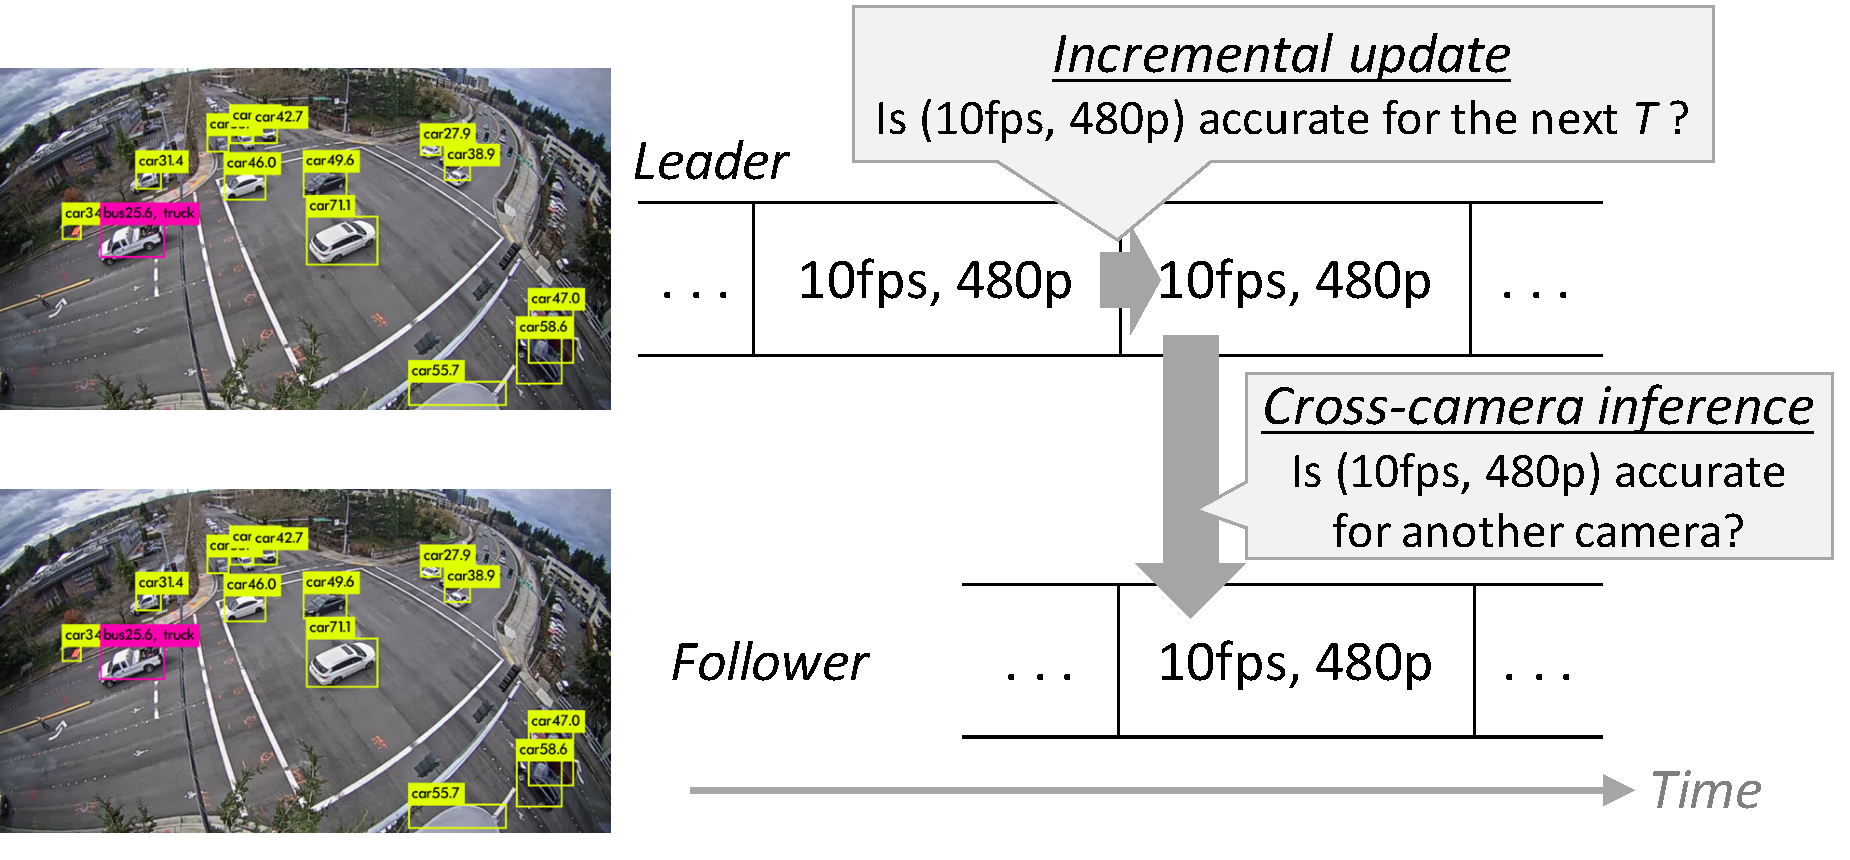
\includegraphics[width=0.5\textwidth]{PaperFigures/Workflow.pdf}
\vspace{-0.2cm}
\tightcaption{Example of how the best configuration of one 
segment is carried over to another segment.}
\label{fig:workflow}
\end{figure}

\name saves the profiling cost for segments between two 
re-profiling events on two fronts:

% Next, we outline the key components in \name to leverage the 
% spatial and temporal correlations in practice. 
% \name splits all available video feeds into {\em segments}, each 
% of which is a set of frames of a video feed in a fine-grained 
% (e.g., one-second) interval. 
% The \nn configurations, however, do not need to be re-profiled 
% and updated on a per segment basis.
% Instead, the temporal and spatial correlation suggests that the 
% best configuration(s) of one segment can be used to ``guide'' the
% of the best configuration of the future segments of the same video 
% and similar videos.
% % Moreover, the spatial correlation suggests that the set of best
% % configurations of one segment should be can guide the selection of
% % the best configuration of the segments of a similar video feed.
% % Therefore,
% Naturally, the design of \name is set to answer two questions:
% \begin{packeditemize}
% \item {\em How to transfer profiles learned in one time window to 
% another?}
% \item {\em How to transfer profiles learned on one video to another?}
% %\item {\em How to efficiently profile the configuration space?}
% \end{packeditemize}

In the rest of the section, we will describe each of the key steps in 
this workflow, namely:
\begin{packedenumerate}
\item How to profile the configuration space once?
\item How to group similar video feeds?
\item How to check the accuracy of another segment's best 
configurations(s) on a different segment?
\end{packedenumerate} 
% The key to their answers is a cost-efficient way of checking 
% whether one-segment's best configuration is good enough for 
% another segment without running any additional configurations.
% The idea here is to use the confidence associated with each 
% detected objects, and establish a correlation between the 
% confidence (which is available instantly and for free) and the
% accuracy (real feedback) just barely strong enough to indicate
% whether the  detected objects, with their confidence, has 
% accuracy over the accuracy threshold. 

% As outlined in Figure~\ref{??}, we can then use this light-weight
% checking on accuracy to decide whether we should re-use the 
% best configuration from the last segment of the same video, or 
% select from the best configurations from a similar video.
% Finally, we still need to re-profile the configuration space 
% once in a while (every tens of seconds) for at least one of the 
% similar video feeds, and an exhaustive search in the 
% configuration space will still blow up the cost. 
% \name address this issue by profiling each knobs separately 
% since these knobs often appear to be independent, thus reducing
% the exponential cost to a linear one.


\subsection{Periodic profiling of configuration spaces}

\name re-profiles the configuration space periodically or
whenever the confidence value changes dramatically.
While this happens relatively infrequently, its cost may
still induce a significant overhead to resource consumption,
especially if the amount of all possible configurations grows
exponentially with more knobs.
Instead of profiling the performance of a high 
dimensional configuration space of multiple knobs, \name
updates one knob at a time while fixing the values on other
knobs.
By treating the knobs separately, we can reduce the 
re-profiling cost from $O(n^k)$ (an exhaustive search in $k$
knobs each having $n$ values) to $O(n\cdot k)$.

%\mypara{Independence among knobs}
Our insight is that 
for each knob, the relationship between its value and inference 
accuracy is independent to the setting on other knobs. 
That is, for instance, if 5fps is the least frame rate to get an F1 
score of 0.8 when the frame size is 960p, then 5fps will be the
least frame rate to attain an F1 score of 0.8 when the frame size 
is 480p.
The intuition behind the independence between knobs is that the 
impact of these knobs on accuracy is determined by {\em orthogonal} 
factors. 
For instance, in pipeline $A$, the frame rate concerns the object
moving speed, image sizes concerns the number of pixels to cover 
each object of interest, and the object detection model depends on 
whether the shape of an object can be expressed by the extracted 
features.
This allows us to profile knobs separately, and safely ignore the 
combinational effects between knobs.

\begin{algorithm}[t!]
\small
	\DontPrintSemicolon
    \SetKwFunction{Overall}{ConfigAdaptation}
    \SetKwFunction{ProfilingUnit}{Profile}
    \SetKwProg{Fn}{Function}{:}{}
	\KwIn{$n$ video feed $M_1,\dots,M_n$, the accuracy threshold $\alpha$, and all possible configurations $C$, each being a combination of values on $k$ knobs, where $V_k$ and $v_k^*$ are the values of knob $k$ and its most expensive value.}
	\KwOut{Configuration $\hat{c}_{M_i,T_j}$ for video $M_i$ in time window $T_j$.}
% 	\Fn{\Overall{$\{M_1,\dots,M_n\}, C, \alpha$}}{
%         \ForEach{$j$-th $T$-second time window $T_j$}{
%     	    \ForEach{$M_i$}{
%         	    $X_{i,j}\leftarrow I(M_i,t_j)$\\
%         	    $\hat{c_{M_i,T_j}}\leftarrow \ProfilingUnit(X_{i,j},C,\alpha)$\\
%         	}
%     	}
%     	\Return{$\hat{c}_{M_i,T_j}$ for all $M_i$ and $T_j$}
% 	}
    \Fn{\ProfilingUnit{$X, C, \alpha$}}{
        $c^{default}=(v_1^{default},\dots,v_m^{default})$\\
        \tcc{\small{Optimize one knob at a time}}
        \ForEach{Knob $k$}{
            $R_{min}\leftarrow\infty$; $A_{best}\leftarrow 1$\\
            \ForEach{$v_k\in V_k$}{
                \tcc{\small{Change only knob $k$ to $v_k$}}
                $c(v_k)\leftarrow Replace(c^{default},k,v_k)$\\
                $c(v_k^*)\leftarrow Replace(c^{default},k,v_k^*)$\\
                $A\leftarrow F(X,c(v_k),c(v_k^*))$\\
                \tcc{\small{Set knob $k$ to $v$, if $v$ is cheaper and is accurate enough}}
                \If{$R(c(v_k)) < R_{min}$ \textrm{\bf and} $A \geq \alpha$}{
                    $\hat{v_k}\leftarrow v$; $R_{min}\leftarrow R(c(v_k))$; $A_{best}\leftarrow A$\\
                }
            }
            \tcc{\small{Update the accuracy threshold}}
            $\alpha=\frac{\alpha}{A_{best}}$
        }
        \Return{$\hat{c}\leftarrow(\hat{v_1},\dots,\hat{v_n})$}
    }
	\caption{Profiling configuration knobs separately.}
	\label{alg:policy3}
\end{algorithm}

%\mypara{Profiling knobs separately}
Algorithm~\ref{alg:policy3} describes how \name profiles the knobs
separately. 
Let $Replace(C,k,v)$ denote the result of setting knob $k$ of $C$ 
with $v$, and $F(X,c,c^*)=\frac{1}{|X|}\sum_{x\in X}f(x,c,c^*)$ 
denote the average F1 score of $c$ with respect to $c^*$ over a 
set of frames $X$.
For every $T$ seconds, it re-profiles and updates the 
configurations on the frames in the first $t$ seconds.
For each knob $k$, it tries all of its possible values while 
fixing other knobs to their default values $C(v_k)$, and calculate
the accuracy with respect to setting knob $k$ to its most 
expensive values as the golden
configuration $C(v_k^*)$ (line~5-7). 
This allow us to identify the ``sweet spot'' value of knob $k$ 
that has least resource consumption while achieving enough 
accuracy (line~8-9).
Finally, since the accuracy degradation of individual knobs will 
be accrued when combining them together, we increase the accuracy 
threshold after each knob is updated (line~10).
% Given a configuration $C$, configuration 
% $C'=C\setminus\{v_k\}\cup \{v_k^*\}$ has the same values to $C$ except for the $k$-th knob, on which $C$ has $v_k$ and $C^*$ has $v_k^*$.
There are two more details in online profiling.
First, for some knobs (e.g., frame rate, minimal area size), a
lower value has no profiling cost, if a higher value has been
profiled, because the output of the lower value can be extrapolated
from the output of a higher values (e.g., for frame rate, it means
simply ignoring frames in the higher frame rate output).
Second, Policy~3 depends on the default values, though different
settings of default values only yield marginal performance 
difference.~\footnote{We notice that such independence would be 
weakened in extreme cases; e.g., it is hard to profile the accuracy
of different frame rates, under too small an image size, as no \nn
would detect any objects. So when profiling a certain knob, other
knobs are not set to such extreme values.}


\subsection{Light-weight checking of accuracy}



